% !TeX spellcheck = pl_PL
\documentclass[a4paper,twoside]{article}
\usepackage{polski}
\usepackage[utf8]{inputenc}
\usepackage{graphicx}
\usepackage{amsmath}

\usepackage[unicode, bookmarks=true]{hyperref} %do zakładek
\usepackage{tabto} % do tabulacji
\NumTabs{6} % globalne ustawienie wielkosci tabulacji
\usepackage{array}
\usepackage{multirow}
\usepackage{array}
\usepackage{dcolumn}
\usepackage{bigstrut}


\setlength{\textheight}{24cm}
\setlength{\textwidth}{15.92cm}
\setlength{\footskip}{10mm}
\setlength{\oddsidemargin}{0mm}
\setlength{\evensidemargin}{0mm}
\setlength{\topmargin}{0mm}
\setlength{\headsep}{5mm}

\newcolumntype{M}[1]{>{\centering\arraybackslash}m{#1}}
\newcolumntype{N}{@{}m{0pt}@{}}

\graphicspath{ {./images/} }

\begin{document}
\bibliographystyle{plain}



\begin{titlepage}
\title{\huge Architektura komputerów - ULTIMATE}
\author{\large SonMati \\ Doxus}
\maketitle
\end{titlepage}

%===============================================================================
% *** PYTANIA I ODPOWIEDZI *****************************************************
%===============================================================================
\part*{Pytania i odpowiedzi}
\section{Moc obliczeniowa komputerów wektorowych :}
	\begin{itemize}
    \item Zależy od liczby stopni potoku
    \item \textbf{Jest odwrotnie proporcjonalna do długości taktu zegarowego}
    \item Jest wprost proporcjonalna do długości taktu zegarowego
    \item Zależy odwrotnie proporcjonalnie od liczby jednostek potokowych połączonych łańcuchowo
    \item \textbf{Zmierza asymptotycznie do wartości maksymalnej wraz ze wzrostem długości wektora}
    \item Nie zależy od długości wektora
    \item Zależy liniowo od długości wektora
    \end{itemize}

\section{Czy poniższa lista jest rosnąco uporządkowana według skalowalności:}
	\begin{itemize}
    \item Systemy ściśle połączone, systemy ze wspólną pamięcią, systemy SMP
    \item \textbf{Systemy ze wspólna magistralą, systemy wielomagistralowe, systemy z przełącznicą krzyżową}
    \item Systemy SMP, systemy z pamięcią wieloportową, systemy z przełącznicą krzyżową
    \item NUMA, MPP, SMP
    \item \textbf{Systemy z pamięcią wspólną, systemy o niejednorodnym dostępie do pamięci, z pamięcią rozproszoną}
    \item Systemy SMP, NUMA, klastry, UMA
    \item \textbf{Systemy symetryczne, o niejednorodnym dostępie do pamięci, systemy z przesyłem komunikatów}
    \end{itemize}
    
\section{Komputery macierzowe}
	\begin{itemize}
    \item \textbf{Mają w liście rozkazów m.in. rozkazy operujące na wektorach danych}
    \item Mają macierzowe potokowe układy arytmetyczne
    \item Mają w typowych rozwiązaniach zestaw pełnych procesów połączonych siecią połączeń
    \item \textbf{Wykonują synchroniczną operację wektorową w sieci elementów przetwarzających}
    \end{itemize}
    
\section{Przetwarzanie potokowe {\small /Forczu}}
	\begin{itemize}
    \item Nie jest realizowane dla operacji zmiennoprzecinkowych\\
    {\small \emph{Nie ma takiego ograniczenia. Przetwarzanie potokowe dotyczy optymalizacji czasu wykonywania rozkazów - podziału realizacji rozkazu na fazy. Owszem, dla argumentów zmiennoprzecinkowym mogą wystąpić problemy związane z czasem obliczeń (uniemożliwienie wykonania rozkazu w jednym takcie), co oże zablokować napełnianie potoku, jednak nie uniemożliwia to zastosowania potoku. /Forczu}}
    \item Nie jest realizowane w procesorach CISC\\
    {\small \emph{Przetwarzanie potokowe znalazło zastosowanie głównie w architekturze RISC, jednak CISC też z niej korzysta. Przykłady: VAX 11/780 (CISC), Ultra SPARC III (RISC)}.}
    \item \textbf{Daje przyspieszenie nie większe od liczby segmentów (stopni) jednostki potokowej}\\
    {\small \emph{Tak, przyspieszenie jest stosunkiem czasu wykonywania \emph{n} rozkazów dla procesora niepotokowego oraz czasu dla procesora potokowego. W idealnym przypadku, gdy każdy stopień dzieli okres rozkazu po równo, a liczba rozkazów dąży do nieskończoności, stosunek ten jest równy P - ilości stopni.}}
    \item W przypadku wystąpienia zależności między danymi wywołuje błąd i przerwanie wewnętrzne.\\
    {\small \emph{Hm, dobre pytanie. Tak, zależnosci danych mogą wystapić (zjawisko hazardu) i rozdupić program, ale po to własnie istnieją mechanizmy by temu zapobiegać. Każda szanująca się architektura to potrafi: albo sprzętowo, albo na etapie kompilacji, która modyfikuje i optymalizuje program. A jeżeli po modyfikacji pewien rozkaz nie wykona się w jednym takcie, napełnianie potoku jest przerywane (ale błędu chyba nie wywala), patrz wyżej.}}
    \item Jest realizowane tylko dla operacji zmiennoprzecinkowych\\
    {\small \emph{Pfff, no chyba nie XD Jest realizowane dla każdego rodzaju rozkazu.}}
    \end{itemize}

% --- PYTANIE 5
\section{W procesorach superskalarnych}
	\begin{itemize}
    \item \textbf{Liczba rozkazów, które procesor może wykonać w 1 takcie zależy od liczby jednostek potokowych w procesorze}
    \item Liczba rozkazów, które procesor może wykonać w jednym takcie, zależy od liczby stopni potoku
    \item Liczba rozkazów pobieranych z pamięci, w każdym takcie musi przekraczać liczbę jednostek potokowych
    \item \textbf{Liczba rozkazów, które procesor może wykonać w taktach zależy od liczby jednostek potokowych w procesorze}
    \end{itemize}

\section{Systemy SMP}
	\begin{itemize}
    \item Wykorzystują protokół MESI do sterowania dostępem do wspólnej magistrali
    \item Posiadają skalowalne procesory
    \item Posiadają pamięć fizycznie rozproszoną, ale logicznie wspólną
    \end{itemize}

\section{Komputery wektorowe}
	\begin{itemize}
    \item Posiadają jednostki potokowe o budowie wektorowej
    \item \textbf{Posiadają w liście rozkazów m.in. rozkazy operujące na wektorach danych}
    \item \textbf{Wykorzystują od kilku do kilkunastu potokowych jednostek arytmetycznych}
    \item Posiadają listę rozkazów operujących wyłącznie na wektorach
    \end{itemize}

\section{Procesory wektorowe}
	\begin{itemize}
    \item \textbf{Mogą być stosowane w systemach wieloprocesorowych}
    \item \textbf{Mają listę rozkazów operującą jedynie na wektorach}
    \item \textbf{Mają moc kilka razy większą od procesorów skalarnych}
    \end{itemize}

\section{Systemy MPP są zbudowane z węzłów którymi mogą być}
	\begin{itemize}
    \item \textbf{Systemy SMP}
    \item Klastry
    \item Konstelacje
    \item \textbf{Systemy NUMA}
    \item \textbf{Procesory}
    \end{itemize}

% --- PYTANIE 10
\section{W architekturze NUMA}
	\begin{itemize}
    \item \textbf{Dane są wymieniane między węzłami w postaci linii pamięci podręcznej (PaP)}
    \item Spójność PaP węzłów jest utrzymywana za pomocą protokołu MESI
    \item Czas dostępu do pamięci lokalnej w węźle jest podobny do czasu dostępu do pamięci nielokalnej
    \item \textbf{Czas zapisu danych do pamięci nielokalnej może być znacznie dłuższy od czasu odczytu z tej pamięci}
    \item \textbf{Każdy procesor ma dostęp do pamięci operacyjnej każdego węzła}
    \item Procesy komunikują się poprzez przesył komunikatów
    \item \textbf{Pamięć operacyjna jest rozproszona fizycznie pomiędzy węzłami, ale wspólna logicznie}
    \end{itemize}

\section{Mechanizmy potokowe stosowane są w celu {\small /Forczu}}
	\begin{itemize}
    \item Uszeregowania ciągu wykonywanych rozkazów\\
    {\small \emph{Nie, zupełnie nie o to chodzi. Ciąg może zostać uszeregowany przez kompilator w celu optymalizacji. Jednak celem tego mechanizmu jest zrównoleglenie wykonywania rozkazów -> zmiana kolejnosci ich realizacji nie jest założeniem.}}
    \item \textbf{Uzyskania równoległej realizacji rozkazów}
    {\small \emph{No tyć. Potoki umożliwiają realizację wielu rozkazów jednoczesnie dzieląc jednostkę centralną na wg stopni, jak np. pobranie rozkazu i wykonania rozkazu. Dzięki temu dwa rozkazy mogą wykonywać się jednoczesnie, oba w innych fazach.}}
    \item \textbf{Przyspieszenia realizacji rozkazów}\\
    {\small \emph{Tak, to główny cel. Umożliwienie wykonania rozkazów umożliwia przyspieszenie, które oblicza się jako stosunek czasu wykonywania rozkazów w procesorze niepotokowym do czasu realizacji w procesorze potokowym. W idealnym przypadku jest ono równe \emph{P} - ilości podziałów / stopni / faz / zwał jak zwał.}}
    \end{itemize}

\section{Protokół MESI}
	\begin{itemize}
    \item Jest wykorzystywany do sterowania dostępem do magistrali w systemie SMP
    \item \textbf{Zapewnia spójność pamięci cache w systemie SMP}
    \item Służy do wymiany komunikatów w systemie MPP
    \item Chroni przed hazardem w proc superskalarnych
    \end{itemize}
    
\section{Mechanizm skoków opóźnionych {\small /Forczu}}
	\begin{itemize}
    \item \textbf{Polega na opóźnianiu wykonywania skoku do czasu wykonania rozkazu następnego za skokiem}\\
    {\small \emph{Tak, cały ten mechanizm sprowadza się do opóźnienia efektu skoku o jeden rozkaz. Zapewnia to, że rozkaz następny po skoku zawsze będzie wykonywany w całosci.}}
    \item Wymaga wstrzymania potoku na jeden takt.\\
    {\small \emph{Nie, mechanizm potoków nie musi być wstrzymywany. Mechanizm ten zmienia postać programu w trakcie kompilacji, ale na samą realizację potoku nie ma wpływu (afaik, not sure).}}
    \item Powoduje błąd na końcu pętli\\
    {\small \emph{Pfff, jak programista ssie pałę to tak, jednak w założeniu tak się nie dzieje.}}
    \item \textbf{Wymaga umieszczenia rozkazu NOP za rozkazem skoku lub reorganizacje programu}.\\
    {\small \emph{Tak, mechanizm sprowadza się do tego, i tylko do tego, patrz pierwsza odpowiedź.}}
    \end{itemize}
    
\section{Charakterystyczne cechy architektury MPP}
	\begin{itemize}
    \item Spójność pamięci podręcznej wszystkich węzłów
    \item \textbf{Fizycznie rozproszona PaO}
    \item Fizycznie rozproszona PaO, ale logicznie wspólna
    \item \textbf{Przesył komunikatów między procesorami}
    \item Niska skalowalność
    \item Jednorodny dostęp do pamięci wszystkich węzłów
    \end{itemize}

% --- PTYTANIE 15
\section{Jak można ominąć hazard danych}
	\begin{itemize}
    \item Poprzez rozgałęzienia
    \item Poprzez uproszczenie adresowania - adresowanie bezpośrednie
    \item \textbf{Przez zamianę rozkazów}
    \end{itemize}

\section{Cechy architektury CISC {\small /Forczu}}
	\begin{itemize}
    \item Czy może być wykonana w VLIW\\
    {\small \emph{Nie, architektura VLIW dotyczy mikroprocesorów i miała na celu jak największe zmniejszenie jednostki centralnej i jej rozkazów (RISC)}. }
    \item \textbf{Czy występuje model wymiany danych typu pamięć - pamięć}\\
    {\small \emph{Tak, posiada róznież niewielką ilosc rejestrow.}}
    \item Jest mała liczba rozkazów\\
    {\small \emph{Nie, w tej architekturze jest PEŁNA (complex) lista rozkazów. Niektóre z zaawansowanych pleceń nawet nie były wykorzystywane, i bum! tak powstał RISC.}}
    \end{itemize}

\section{Cechy architektury RISC {\small /Forczu}}
	\begin{itemize}
    \item \textbf{Czy występuje model wymiany danych typu rej-rej}\\
    {\small \emph{Tak, a komunikacja z pamięcią operacyjną odbywa się wyłącznie za pomocą rozkazów LOAD i STORE}}
    \item \textbf{Jest mała liczba trybów adresowania}\\
    {\small \emph{Tak, raptem 4 w procesorze RISC I podczas gdy CISCi mogą mieć ich kilkanascie, w tym takie bardzo złożone.}}
    \item \textbf{Jest wykonywanych kilka rozkazów w jednym takcie}\\
    {\small \emph{Tu jest haczyk - pierwszy procesor RISC I (1980) stawiał sobie za cel wykonanie \emph{jednego rozkazu w jednym takcie} i dokładnie tak brzmiało jego założenie projektowe. Jednak jego fizyczna realizacja (1982) posiadała dwustopniowy potok.}}
    \item \textbf{Jest wykonywanych kilka rozkazów w jednym takcie (w danej chwili czasu)}\\
    {\small \emph{Chodzi o przetwarzanie potokowe. Patrz wyżej + w wykładach jako cecha tej architektury jest napisane "Intensywne wykorzystanie przetwarzania potokowego", co odnosi się do faktu, że obecnie nie ma procesora typu RISC, który go nie ma. Wg mnie prawda.}}
    \item Jest wykonywanych kilka instrukcji procesora w jednym rozkazie asemblerowym\\
    {\small \emph{Nic mi na ten temat nie wiadomo. Brzmi jednak zbyt hardo i odlegle od tematu zmniejszania ilosci rozkazów.}}
    \item \textbf{Układ sterowania w postaci logiki szytej}\\
    {\small \emph{Tak.}}
    \end{itemize}

\section{Przepustowość (moc obliczeniowa) dużych komputerów jest podawana w}
	\begin{itemize}
    \item \textbf{GFLOPS}
    \item Liczbie instrukcji wykonywanych na sekundę
    \item \textbf{Liczbie operacji zmiennoprzecinkowych na sekundę}
    \item Mb/sek
    \end{itemize}

\section{Podstawą klasyfikacji Flynna jest}
	\begin{itemize}
    \item Liczba jednostek przetwarzających i sterujących w systemach komputerowych
    \item Protokół dostępu do pamięci operacyjnej
    \item \textbf{Liczba strumieni rozkazów i danych w systemach komputerowych}
    \item Liczba modułów pamięci operacyjnej w systemach komputerowych
    \end{itemize}

% --- PYTANIE 20
\section{Liczba modułów pamięci operacyjnej w systemach komputerowych}
	\begin{itemize}
    \item \textbf{Macierzy elementów przetwarzających}
    \item Zestawu procesorów superskalarnych
    \item \textbf{Technologii MMX}
    \item Sieci połączeń typu krata
    \item \textbf{Potokowych jednostek arytmetycznych}
    \end{itemize}

\section{Architektura superskalarna}
	\begin{itemize}
    \item Dotyczy systemów SMP
    \item Wymaga zastosowania protokołu MESI
    \item \textbf{Umożliwia równoległe wykonywanie kilku rozkazów w jednym procesorze}
    \item Wywodzi się z architektury VLIW
    \end{itemize}

\section{Klastry}
	\begin{itemize}
    \item Mają średnią skalowalność
    \item Wykorzystują model wspólnej pamięci
    \item \textbf{W węzłach mogą wykorzystywać systemy SMP}
    \item \textbf{Do komunikacji między procesami wykorzystują przesył komunikatów}
    \item Wykorzystują przełącznicę krzyżową jako sieć łączącą węzły
    \item \textbf{W każdym węźle posiadają pełną instalację systemu operacyjnego}
    \end{itemize}

\section{Pojęcie równoległości na poziomie rozkazów:}
	\begin{itemize}
    \item Dotyczy architektury MIMD
    \item \textbf{Odnosi się m.in. do przetwarzania potokowego}\\
    {\small \emph{Tak, ideą mechanizmu potoków jest zrównoleglenie rozkazów i możliwosć wykonywania wielu z nich w tej samej chwili czasu.}}
    \item Dotyczy architektury MPP
    \item \textbf{Dotyczy m.in. architektury superskalarnej}
    \end{itemize}

\section{Systemy wieloprocesorowe z pamięcią wspólną}
	\begin{itemize}
    \item Zapewniają jednorodny dostęp do pamięci
    \item \textbf{Mogą wykorzystywać procesory CISC}
    \item \textbf{Są wykorzystywane w klastrach}
    \item Wykorzystują przesył komunikatów między procesorami
    \item \textbf{Wykorzystują katalog do utrzymania spójności pamięci podręcznych}
    \end{itemize}

% --- PYTANIE 25
\section{Hazard danych {\small /Forczu}}
	\begin{itemize}
    \item \textbf{Czasami może być usunięty przez zmianę kolejności wykonania rozkazów}\\
    {\small \emph{Tak, służy do tego mechanizm skoków opóżnionych, który odbywa się na poziomie kompilacji programu.}}
    \item Nie występuje w architekturze superskalarnej
    \item Jest eliminowany przez zastosowanie specjalnego bitu w kodzie programu\\
    {\small \emph{Nic mi o tym nie wiadomo. Pewne dodatkowe bity są wykorzystywane w mechaniźmie przewidywania rozgałęzień, który służy do eliminacji hazardu, jednak on to odbywa się PRZED realizacją programu i sprowadza się do zmiany kolejnosci wykonywania rozkazów przez kompilator. Nic nie dodaje do tresci programu.}}
    \item Może wymagać wyczyszczenia potoku i rozpoczęcia nowej (…)\\
    {\small \emph{Nie wiem jak hazard danych może czegokolwiek wymagać skoro jest zjawiskiem ubocznym i je eliminujemy. Jeżeli jednak chodzi o metody eliminacji hazardu, jak mechanizmy skoków opóźnionych lub przewidywania rozgałęzień, nie wymagają czyszczenia potoku. Sprzetowa i programowa eliminacja hazardu jedynie może doprowadzić do \textbf{wstrzymania} napełniania potoku.}}
    \end{itemize}

\section{Przetwarzanie wielowątkowe}
	\begin{itemize}
    \item \textbf{Zapewnia lepsze wykorzystanie potoków}
    \item \textbf{Minimalizuje straty wynikające z chybionych odwołań do pamięci podręcznej}
    \item \textbf{Wymaga zwielokrotnienia zasobów procesora (rejestry, licznik rozkazów...)}
    \item Nie może być stosowane w przypadku hazardu danych
    \end{itemize}

\section{Okna rejestrów {\small /Forczu}}
	\begin{itemize}
    \item Chronią przez hazardem danych\\
    {\small \emph{Lolnope, od tego są mechanizmy skoków opóźnionych i przewidywania rozgałęzień. Okno rejestrów zapewnia ciągłe i optymalne wykonywanie procedur.}}
    \item \textbf{Minimalizują liczbę odwołań do pamięci operacyjnej przy operacjach wywołania procedur}\\
    {\small \emph{Tak, dokładnie do tego one służą. Rejestr niski procedury A staje się rejestrem wysokim procedury B itd. Innymi słowy, procedura A wywołuje procedurę B, i tak dalej. I po cos w tym wszystkim są rejestry globalne.}}
    \item Są charakterystyczne dla architektury CISC\\
    {\small \emph{Nie, zostały zaprojektowane specjalnie dla architektury RISC. Jako pierwszy posiadał je procesor RISC I.}}
    \item Są zamykane po błędnym przewidywaniu wykonania skoków warunkowych.\\
    {\small \emph{W mechanizmie prognozowania rozgałęzień jest możliwosć błędnego przewidywania. Jednak błędna prognoza powoduje tylko zmianę strategii (przewidywanie wykonania lub niewykonania), a nie zamykanie okna.}}
    \item \textbf{Są przesuwane przy operacjach wywołania procedur}\\
    {\small \emph{Tak, z każdą nową wywołaną procedurą okno rejestrów przesuwane jest w dół (ze 137 do 0)}}
    \end{itemize}

\section{Tablica historii rozgałęzień {\small /Forczu}}
	\begin{itemize}
    \item \textbf{Zawiera m.in. adresy rozkazów rozgałęzień}\\
    {\small \emph{Tak, tablica ta zawiera bit ważnosci, \emph{adres rozkazu rozgałęzienia}, bity historii oraz \emph{adres docelowy rozgałęzienia}.}}
    \item \textbf{Pozwala zminimalizować liczbę błędnych przewidywań rozgałęzień w zagnieżdżonej pętli}\\
    {\small \emph{Tak, z tego co wiem jest strategią dynamiczną i najbardziej optymalną ze wszystkich - skończony automat przewidywania rozgałęzień oparty na tej tablicy (z dwoma bitami historii) może być zarealizowany na dwóch bitach.}}
    \item Nie może być stosowana w procesorach CISC\\
    {\small \emph{Ten mechanizm służy zabezpieczeniu przed hazardem, który występuje w przetwarzeniu potokowym, a z tego korzystają zarówn CISC jak i RISC.}}
    \item Jest obsługiwana przez jądro systemu operacyjnego\\
    {\small \emph{Chyba nie, ten mechanizm znajduje się w kompilatorze.}}
    \end{itemize}

\section{Rozkazy wektorowe}
	\begin{itemize}
    \item Nie mogą być wykonywane bez użycia potokowych jednostek arytmetycznych
    \item \textbf{W komputerach wektorowych ich czas wykonania jest wprost proporcjonalny do długości wektora}
    \item \textbf{Są charakterystyczne dla architektury SIMD}
    \item Są rozkazami dwuargumentowymi i w wyniku zawsze dają wektor
    \end{itemize}

% --- PYTANIE 30
\section{Model SIMD}
	\begin{itemize}
    \item Był wykorzystywany tylko w procesorach macierzowych
    \item \textbf{Jest wykorzystywany w multimedialnych rozszerzeniach współczesnych procesorów}
    \item \textbf{Jest wykorzystywany w heterogenicznej architekturze PowerXCell}
    \item \textbf{Zapewnia wykonanie tej samej operacji na wektorach argumentów}
    \end{itemize}

\section{Przesył komunikatów}
	\begin{itemize}
    \item \textbf{Ma miejsce w systemach MPP}
    \item W systemach MPP II-giej generacji angażuje wszystkie procesory na drodze przesyłu
    \item \textbf{Ma miejsce w klastrach}
    \end{itemize}

\section{Cechami wyróżniającymi klastry są}
	\begin{itemize}
    \item \textbf{niezależność programowa każdego węzła}
    \item Fizycznie rozproszona, ale logicznie wspólna pamięć operacyjna
    \item Nieduża skalowalność
    \item \textbf{Na ogół duża niezawodność}
    \end{itemize}

\section{Systemy wieloprocesorowe z pamięcią rozproszoną}
	\begin{itemize}
    \item Wyróżniają się bardzo dużą skalowalnością
    \item Są budowane z węzłów, którymi są klastry
    \item \textbf{Realizują synchronicznie jeden wspólny program}
    \item Wymagają zapewnienia spójności pamięci podręcznych pomiędzy węzłami
    \end{itemize}

\section{Problemy z potokowym wykonywaniem rozkazów skoków (rozgałęzień) mogą być wyeliminowane lub ograniczone przy pomocy}
	\begin{itemize}
    \item Zapewnienia spójności pamięci podręcznej
    \item \textbf{Tablicy historii rozgałęzień}\\
    {\small \emph{Tak, to najprawdopodobniej najlepszy służący ku temu mechanizm. Stara się przewidywać czy skok będzie wykonany bądź nie, wykorzystuje do tego kilka strategii.}}
    \item Techniki wyprzedzającego pobrania argumentu\\
    {\small \emph{Nie, ten mechanizm służy do eliminacji hazardu danych - zależnosci między argumentami.}}
    \item \textbf{Wystawienia do programu rozkazów typu „nic nie rób”}\\
    {\small \emph{Tak, tym rozkazem jest \emph{NOP} i jest wstawiany przez mechanizm skoków opóźnionych, który służy do zabezpieczania potoku.}}
    \item Protokołu MESI
    \item \textbf{Wykorzystania techniki skoków opóźniających}\\
    {\small \emph{Tak, umożliwiają ona modyfikację programu (wstawienie rozkazu NOP), albo jego optymalizację (zamiana kolejnosci wykonywania rozkazów.) Mechanizm ten opóźnia efekt skoku o jeden rozkaz, co zapewnia, że rozkaz po skoku będzie w całosci wykonany.}}
    \item Technologii MMX
    \end{itemize}

% --- PYTANIE 35
\section{W architekturze ccNUMA}
	\begin{itemize}
    \item \textbf{Każdy procesor ma dostęp do pamięci operacyjnej każdego węzła}
    \item Spójność pamięci pomiędzy węzłami jest utrzymywana za pomocą protokołu MESI
    \item \textbf{Dane są wymieniane między węzłami w postaci linii pamięci podręcznej}
    \item \textbf{Pamięć operacyjna jest fizycznie rozproszona pomiędzy węzłami, ale wspólna logicznie}
    \end{itemize}

\section{Dla sieci systemowych (SAN) są charakterystyczne}
	\begin{itemize}
    \item \textbf{Przesył komunikatów w trybie zdalnego DMA}
    \item \textbf{Bardzo małe czasy opóźnień}
    \item Topologia typu hipersześcian
    \item Niska przepustowość
    \end{itemize}

\section{W systemach wieloprocesorowych katalog służy do}
	\begin{itemize}
    \item Śledzenia adresów w protokole MESI
    \item Sterowania przesyłem komunikatów
    \item \textbf{Utrzymania spójności pamięci w systemach o niejednorodnym dostępie do pamięci}
    \item \textbf{Realizacji dostępu do nielokalnych pamięci w systemach NUMA}
    \end{itemize}

\section{W procesorach superskalarnych}
	\begin{itemize}
    \item \textbf{Jest możliwe równoległe wykonywanie kilku rozkazów w jednym procesorze(rdzeniu) }
    \item \textbf{Rozszerzenia architektury wykorzystujące model SIMD umożliwiają wykonanie rozkazów wektorowych}
    \item Nie występuje prawdziwa zależność danych
    \item \textbf{Mogą wystąpić nowe formy hazardu danych: zależności wyjściowe między rozkazami oraz antyzależności}
    \end{itemize}

\section{Efektywne wykorzystanie równoległości na poziomie danych umożliwiają}
	\begin{itemize}
    \item \textbf{Komputery wektorowe}
    \item \textbf{Komputery macierzowe}
    \item \textbf{Klastry}
    \item \textbf{Procesory graficzne}
    \item \textbf{Rozszerzenia SIMD procesorów superskalarnych}
    \end{itemize}

% --- PYTANIE 40
\section{Wielowątkowość współbieżna w procesorze wielopotokowym zapewnia}
	\begin{itemize}
    \item \textbf{Możliwość wprowadzenia rozkazów różnych wątków do wielu potoków}
    \item \textbf{Realizację każdego z wątków do momentu wstrzymania któregoś rozkazu z danego wątku}
    \item Przełączanie wątków co takt
    \item Automatyczne przemianowanie rejestrów
    \end{itemize}

\section{Architektura CUDA}
	\begin{itemize}
    \item \textbf{Umożliwia bardzo wydajne wykonywanie operacji graficznych}
    \item \textbf{Stanowi uniwersalną architekturę obliczeniowa połączoną z równoległym modelem programistycznym}
    \item \textbf{Realizuje model obliczeniowy SIMT}
    \item Jest podstawą budowy samodzielnych, bardzo wydajnych komputerów
    \end{itemize}

\section{Spójność pamięci podręcznych w procesorze wielordzeniowym może być m.in. zapewniona za pomocą}
	\begin{itemize}
    \item Przełącznicy krzyżowej
    \item Katalogu
    \item \textbf{Protokołu MESI}
    \item Wspólnej magistrali
    \end{itemize}

\section{Metoda przemianowania rejestrów jest stosowana w celu eliminacji}
	\begin{itemize}
    \item Błędnego przewidywania rozgałęzień
    \item Chybionego odwołania do pamięci podręcznej
    \item Prawdziwej zależności danych
    \item \textbf{Zależności wyjściowej między rozkazami}
    \item \textbf{Antyzależności między rozkazami}
    \end{itemize}

\section{W systemach wieloprocesorowych o architekturze CC-NUMA}
	\begin{itemize}
    \item \textbf{Spójność pamięci wszystkich węzłów jest utrzymywana za pomocą katalogu}
    \item \textbf{Pamięć operacyjna jest rozproszona fizycznie pomiędzy węzłami, ale wspólna logicznie}
    \item Każdy procesor ma bezpośredni dostęp do pamięci operacyjnej każdego węzła
    \item Dane są wymieniane między węzłami w postaci linii pamięci podręcznej
    \end{itemize}

% --- PYTANIE 45
\section{W tablicy historii rozgałęzień z 1 bitem historii można zastosować następujący algorytm przewidywania (najbardziej złożony)}
	\begin{itemize}
    \item Skok opóźniony\\
    {\small \emph{Nie, skoki opóźnione nie służą do przewidywania rozgałęzień, są zupełnie innym mechanizmem eliminacji hazardu.}}
    \item Przewidywanie, że rozgałęzienie (skok warunkowy) zawsze nastąpi\\
    {\small \emph{Nie, to strategia statyczna, która może być wykonywana gdy adres rozkazu rozgałęzienia NIE jest w tablicy. Nie wykorzystuje bitu historii.}}
    \item Przewidywanie, że rozgałęzienie nigdy nie nastąpi\\
    {\small \emph{Nie, to strategia statyczna, która może być wykonywana gdy adres rozkazu rozgałęzienia NIE jest w tablicy. Nie wykorzystuje bitu historii.}}
    \item \textbf{Przewidywanie, że kolejne wykonanie rozkazu rozgałęzienia będzie przebiegało tak samo jak poprzednie}\\
    {\small \emph{Tak, i to jest wszystko na co stać historię 1-bitową. Historia 2-bitowa umożliwia interepretację:
    		\begin{itemize}
    			\item historii ostatniego wykonania skoku - tak lub nie
    			\item przewidywania następnego wykonania skoku - tak lub nie
    		\end{itemize}
    		A zamiana strategii następuje dopiero po drugim błędzie przewidywania.}}
    \item Wstrzymanie napełniania potoku\\
    {\small \emph{Nie, wstrzymywanie potoku mogą spowodować algorytmy zajmujące się eliminacją hazardu danych - zależnosci między argumentami.}}
    \end{itemize}

\section{Do czynników tworzących wysoką niezawodność klastrów należą}
	\begin{itemize}
    \item \textbf{Mechanizm mirroringu dysków}
    \item \textbf{Dostęp każdego węzła do wspólnych zasobów(pamięci zewnętrznych)}
    \item \textbf{Redundancja węzłów}
    \item Mechanizm "heartbeat"
    \item Zastosowanie procesorów wielordzeniowych w węzłach
    \end{itemize}

\newpage
%===============================================================================
%*******************************************************************************
%===============================================================================
\part*{Opracowanie wykładów}
\section*{Historia rozwoju komputerów}
	\begin{enumerate}
    \item Liczydło
    \item Pascalina - maszyna licząca Pascala (dodawanie i odejmowanie)
    \item Maszyna mnożąca Leibniza (dodawanie, odejmowanie, mnożenie, dzielenie, pierwiastek kwadratowy
    \item Maszyna różnicowa - Charles Babbage, obliczanie wartości matematycznych do tablic
    \item Maszyna analityczna - Charles Babvage, programowalna za pomocą kart perforowanych
  	\item Elektryczna maszyna sortująca i tabelaryzująca Holleritha 1890
    \item Kalkulator elektromechaniczny Mark I, tablicowanie funkcji, całkowanie numeryczne, rozwiązywanie równań różniczkowych, rozwiązywanie układów równań liniowych, analiza harmoniczna, obliczenia statystyczne
    \item Maszyny liczące Z1: pamięć mechaniczna, zmiennoprzecinkowa reprezentacja liczb, binarna jednostka zmiennoprzecinkowa
    \item Z3: Pierwsza maszyna w pełni automatyczna, kompletna w sensie Turinga, pamięć przekaźnikowa
    \item Colossus i Colossus 2
    \item ENIAC
    \item EDVAC - J. von Neumann (wtedy utworzył swoją architekturę) \\
    	\begin{figure}[h]
		\centering
		%\includegraphics[scale=0.1]{architektura_von_Neumanna.png}
		\end{figure}
    \item UNIVAC I (pierwszy udany komputer komercyjny)
    \item IBM 701, potem 709
    \item po 1955 zaczyna się zastosowanie tranzystorów w komputerach (komputery II generacji)
    \item po 1965 komputery III generacji z układami scalonymi
    \item od 1971 komputery IV generacji - z układami scalonymi wielkiej skali inegracji VLSI
    \end{enumerate}
    
    
    
\section*{Architektura CISC}
	\subsection*{Znaczenie} \noindent
	Complex Instruction Set Computers
	
	\subsection*{Przyczyny rozwoju architektury CISC}
    	\begin{itemize}
        \item Drogie, małe i wolne pamięci komputerów
        \item Rozwój wielu rodzin komputerów
        \item Duża popularność mikroprogramowalnych układów sterujących (prostych w rozbudowie)
        \item Dążenie do uproszczenia kompilatorów. Im więcej będzie rozkazów maszynowych odpowiadających instrukcjom języków wyższego poziomu tym lepiej.
        \end{itemize}
    
    \subsection*{Cechy architektury CISC}
    	\begin{itemize}
        \item Duża liczba rozkazów (z czego te najbardziej zaawansowane i tak nie były używane)
        \item Duża ilość trybów adresowania (związane z modelem obliczeń)
        \item Duży rozrzut cech rozkazów w zakresie:
        \begin{itemize}
	        \item złożoności
	        \item długości (szczególnie to - nawet kilkanaście bajtów)
	        \item czasów wykonania
        \end{itemize}
        \item Model obliczeń pamięć - pamięć
        \item Niewiele rejestrów - były droższe niż komórki pamięci i przy przełączaniu kontekstu obawiano się wzrostu czasu przełączania kontekstu (chowanie rejestrów na stos i odwrotnie)
        \end{itemize}
   
   \textbf{\large CIEKAWOSTKA:} Przeanalizowano jakieś tam programy i w procesorze VAX 20\% najbardziej złożonych rozkazów odpowiadało za 60\% kodu, stanowiąc przy tym ok 0.2\% wywołań.\\ W procesorze MC68020 71\% rozkazów nie zostało nawet użytych w badanych programach
   
	\section*{Architektura RISC}
		\subsection*{Znaczenie} \noindent
		Reduced Instruction Set Computers
   		\subsection*{Przyczyny rozwoju}
   		\begin{itemize}
   			\item Poszukiwanie optymalnej listy rozkazów
   			\item Chęć wykonania mikroprocesora o funkcjach pełnego ówczesnego procesora
   		\end{itemize}
   		
   		\subsection*{Pierwszy procesor RISC} \noindent
   		Procesor RISC I (1980), D. Patterson (Berkeley University)\\
   		Założenia projektowe:
   		\begin{itemize}
   			\item Wykonanie jednego rozkazu w jednym cyklu maszynowym
   			\item Stały rozmiar rozkazów – uproszczenie metod adresacji
   			\item Model obliczeń rejestr – rejestr: komunikacja z pamięcią operacyjną tylko za pomocą rozkazów LOAD i STORE.
   			\item Wsparcie poprzez architekturę języków wysokiego poziomu.
   		\end{itemize}
   		Efekty realizacji fizycznej:
   		\begin{itemize}
   			\item 44 420 tranzystorów (ówczesne procesory CISC zawierały ok. 100 000 tranzystorów)
   			\item lista rozkazów = 32 rozkazy
   			\item dwustopniowy potok – strata tylko 6\% cykli zegara, zamiast 20\% (w związku z realizacją skoków)
   		\end{itemize}
   		
   		\subsection*{Cechy architektury RISC}
   		\begin{enumerate}
   			\item Stała długość i prosty rozkaz formatu
   			\item Nieduża liczba trybów adresowania
   			\item Niezbyt obszerna lista rozkazów
   			\item Model obliczeń rejestr-rejestr - dostęp do pamięci operacyjnej tylko w rozkazach LOAD i STORE
   			\item Duży zbiór rejestrów uniwersalnych
   			\item Układ sterowania – logika szyta
   			\item Intensywne wykorzystanie przetwarzania potokowego
   			\item Kompilatory o dużych możliwościach optymalizacji potoku rozkazów
   		\end{enumerate}
   		
   		
   		\subsection*{Format rozkazu procesora RISC I}
   		\begin{table}[h]
   			\begin{tabular}{clclll}
   				\hline
   				\multicolumn{1}{|c|}{7}      & \multicolumn{1}{c|}{1}   & \multicolumn{1}{c|}{5}    & \multicolumn{1}{c|}{5}    & \multicolumn{1}{c|}{1}   & \multicolumn{1}{c|}{13}   \\ \hline
   				\multicolumn{1}{|c|}{OPCODE} & \multicolumn{1}{c|}{SCC} & \multicolumn{1}{c|}{DEST} & \multicolumn{1}{c|}{SRC1} & \multicolumn{1}{c|}{IMM} & \multicolumn{1}{c|}{SRC2} \\ \hline
   			\end{tabular}
   		\end{table}
   		\begin{itemize}
   			\item OPCODE–kod rozkazu
   			\item SCC – ustawianie (lub nie) kodów warunków
   			\item DEST – nr rejestru wynikowego
   			\item SRC1 – nr rejestru zawierającego pierwszy argument
   			\item IMM – wskaźnik natychmiastowego trybu adresowania
   			\item SRC2 – drugi argument lub nr rejestru (na 5 bitach)
   		\end{itemize}
   		
   		\subsection*{Realizacja wybranych rozkazów}
   			\subsubsection*{Rozkazy arytmetyczne}
   			\begin{itemize}
   				\item \textbf{Tryb rejestrowy}:\tab(IMM=0) \tab R[DEST] $\leftarrow$ R[SRC1] op R[SRC2]
   				\item \textbf{Tryb natychmiastowy:}\tab(IMM=1) \tab{R[DEST] $\leftarrow$ R[SRC1] op SRC2}
  			\end{itemize}
        	\subsubsection*{Rozkazy komunikujące się z pamięcią}
        	\begin{itemize}
        		\item \textbf{LOAD}\tab{R[DEST] $\leftarrow$ M[AE]P}
        		\item \textbf{STORE}\tab{M[AE]  $\leftarrow$ R[DEST]}
        	\end{itemize}
        	\subsubsection*{Adres efektywny}
        	\begin{itemize}
        		\item \textbf{Tryb z przesunięciem}\tab\tab AE = R[SRC1] + SRC2 = RX + S2
        		\item \textbf{Inny zapis powyższego}\tab\tab AE = RX + S2
        		\item \textbf{Tryb absolutny}\tab\tab AE = R0 + S2 = S2 (R0 $\equiv$ 0)
        		\item \textbf{Tryb rejestrowy pośredni}\tab AE = RX + 0 = RX
        	\end{itemize}
        	Tryb absolutny oraz tryb rejestrowy pośredni są przypadkami szczególnymi.
        	
    \subsection*{Logiczna organizacja rejestrów procesora RISC I}
	    \begin{table}[htbp]
	    	\centering
	    	\caption{Rejestry}
	    	\begin{tabular}{c|c|c}
	    		\cline{2-2}    \multirow{4}[2]{*}{6} & \multirow{4}[2]{*}{Wysokie} & {\scriptsize R31} \bigstrut[t]\\
	    		&       &  \\
	    		&       &  \\
	    		&       &  \bigstrut[b]\\
	    		\cline{2-2}    \multirow{4}[2]{*}{10} & \multirow{4}[2]{*}{Lokalne} &  \bigstrut[t]\\
	    		&       &  \\
	    		&       &  \\
	    		&       &  \bigstrut[b]\\
	    		\cline{2-2}    \multirow{4}[2]{*}{6} & \multirow{4}[2]{*}{Niskie} &  \bigstrut[t]\\
	    		&       &  \\
	    		&       &  \\
	    		&       &  \bigstrut[b]\\
	    		\cline{2-2}    \multirow{4}[2]{*}{10} & \multirow{4}[2]{*}{Globalne} & {\scriptsize R9} \bigstrut[t]\\
	    		&       &  \\
	    		&       &  \\
	    		&       & {\scriptsize R0} \bigstrut[b]\\
	    		\cline{2-2}    \end{tabular}%
	    	\label{tab:addlabel}%
	    \end{table}%
	    \subsection*{Okno rejestrów}
	    \begin{table}[htbp]
	    	\centering
	    	\caption{Rejestry fizyczne}
	    	\begin{tabular}{r|r|r}
	    		\cline{2-2}    137   & \multirow{6}[2]{*}{$ \uparrow $ Okno rejestrów} &  \bigstrut[t]\\
	    		&       &  \\
	    		&       &  \\
	    		&       &  \bigstrut[b]\\
	    		\cline{2-2}          & \multicolumn{1}{c|}{\multirow{4}[2]{*}{Wysokie}} & \multicolumn{1}{c}{R31} \bigstrut[t]\\
	    		& \multicolumn{1}{c|}{} & \multicolumn{1}{c}{} \\
	    		& \multicolumn{1}{c|}{} & \multicolumn{1}{c}{} \\
	    		& \multicolumn{1}{c|}{} & \multicolumn{1}{c}{} \bigstrut[b]\\
	    		\cline{2-2}          & \multicolumn{1}{c|}{\multirow{4}[2]{*}{Lokalne}} & \multicolumn{1}{c}{} \bigstrut[t]\\
	    		& \multicolumn{1}{c|}{} & \multicolumn{1}{c}{} \\
	    		& \multicolumn{1}{c|}{} & \multicolumn{1}{c}{} \\
	    		& \multicolumn{1}{c|}{} & \multicolumn{1}{c}{} \bigstrut[b]\\
	    		\cline{2-2}          & \multicolumn{1}{c|}{\multirow{4}[2]{*}{Niskie}} & \multicolumn{1}{c}{} \bigstrut[t]\\
	    		& \multicolumn{1}{c|}{} & \multicolumn{1}{c}{} \\
	    		& \multicolumn{1}{c|}{} & \multicolumn{1}{c}{} \\
	    		& \multicolumn{1}{c|}{} & \multicolumn{1}{c}{} \bigstrut[b]\\
	    		\cline{2-2}          & \multicolumn{1}{c|}{\multirow{4}[2]{*}{Globalne}} & \multicolumn{1}{c}{} \bigstrut[t]\\
	    		& \multicolumn{1}{c|}{} & \multicolumn{1}{c}{} \\
	    		& \multicolumn{1}{c|}{} & \multicolumn{1}{c}{} \\
	    		& \multicolumn{1}{c|}{} & \multicolumn{1}{c}{R0} \bigstrut[b]\\
	    		\cline{2-2}          & \multicolumn{1}{c|}{\multirow{2}[2]{*}{$ \downarrow $ }} &  \bigstrut[t]\\
	    		& \multicolumn{1}{c|}{} &  \\
	    		0     & \multicolumn{1}{c|}{} &  \bigstrut[b]\\
	    		\cline{2-2}    \end{tabular}%
	    	\label{tab:addlabel}%
	    \end{table}
	    
	    % --- OBRAZKI
%	    \begin{center}
%	    	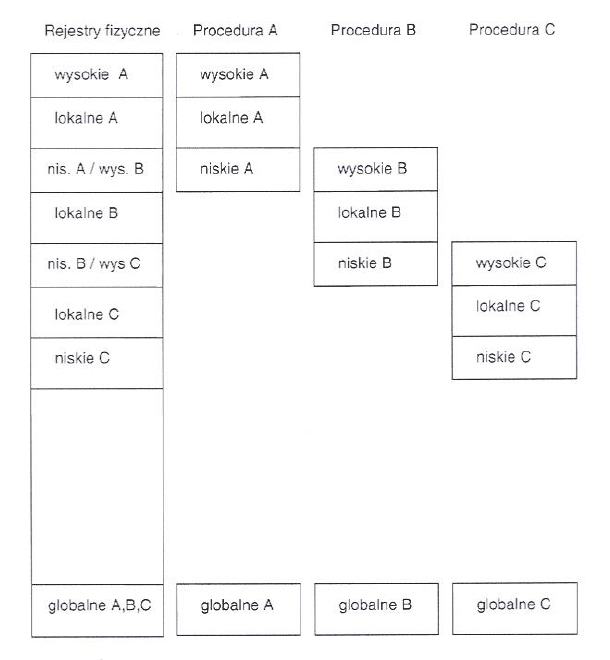
\includegraphics[width=10cm]{RISC_proc1}
%	    \end{center}
%	    \begin{center}
%	    	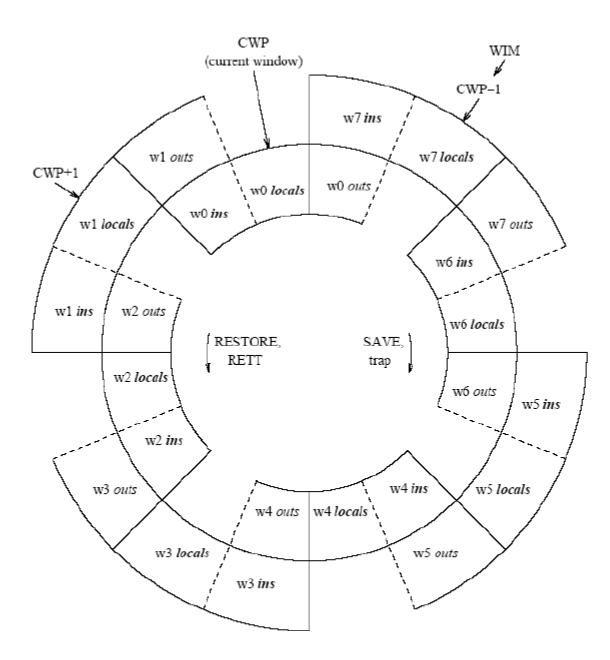
\includegraphics[width=10cm]{RISC_proc2}
%	    \end{center}
	    
	\pagebreak
	\section*{Mechanizmy potokowe}
		\subsection*{Realizacja rozkazów w procesorze niepotokowym}
		Rozkazy wykonywane są liniowo w czasie - jeden po drugim, w takiej kolejności w jakiej przyjdą do procesora.
    	\subsection*{Potokowe wykonanie rozkazówdla prostej organizacji cyklu rozkazowego}
    	Prosty podział procesora na moduły:
    	\begin{itemize}
    		\item S1 - pobranie rozkazu
    		\item S2 - wykonanie rozkazu
    	\end{itemize}
    	Zakładając, że czas pracy obu modułów jest równy, wówczas 3 rozkazy mogą zostać wykonane w 2 okresach.\\
    	1 T - pobranie i wykonanie rozkazu. W momencie gdy pierwszy rozkaz zostanie pobrany, w chwili 0.5 T S1 może pobrać kolejny.
    	\subsection*{Podział cyklu rozkazowego na większą liczbę faz}
    	Na przykładzie cyklu rozkazowego komputera Amdahl 470
    	\begin{enumerate}
    		\item Pobranie rozkazu
    		\item Dekodowanie rozkazu
    		\item Obliczenie adresu efektywnego
    		\item Pobranie argumentów
    		\item Wykonanie operacji
    		\item Zapis wyniku
    	\end{enumerate}
    	Zasada działania jest dokładnie taka sama jak w przypadku podziału na dwie fazy. Załóżmy, że jeden rozkaz wykonuje się w 7iu taktach zegarowych. 1 T = 7 F. Wówczas w momencie gdy rozkaz numer 1 znajduje się w 5tym takcie wykonania rozkaz numer 5 może zostać pobrany.
    	% Table generated by Excel2LaTeX from sheet 'Arkusz1'
    	\begin{table}[htbp]
    		\centering
    		\caption{Zobrazowanie potoku}
    		\begin{tabular}{|r|r|r|r|r|r|r|r|r|}
    			\multicolumn{1}{r}{Rozkazy} & \multicolumn{1}{r}{} & \multicolumn{7}{c}{Fazy zegarowe} \\
    			\multicolumn{1}{r}{} & \multicolumn{1}{r}{} & \multicolumn{1}{c}{1} & \multicolumn{1}{c}{2} & \multicolumn{1}{c}{3} & \multicolumn{1}{c}{4} & \multicolumn{1}{c}{5} & \multicolumn{1}{c}{6} & \multicolumn{1}{c}{7} \bigstrut[b]\\
    			\cline{1-1}\cline{3-9}    \multicolumn{1}{|c|}{S1} &       & r1    & r2    & r3    & r4    & r5    & r6    & r7 \bigstrut\\
    			\cline{1-1}\cline{3-9}    \multicolumn{1}{|c|}{S2} &       &       & r1    & r2    & r3    & r4    & r5    & r6 \bigstrut\\
    			\cline{1-1}\cline{3-9}    \multicolumn{1}{|c|}{S3} &       &       &       & r1    & r2    & r3    & r4    & r5 \bigstrut\\
    			\cline{1-1}\cline{3-9}    \multicolumn{1}{|c|}{S4} &       &       &       &       & r1    & r2    & r3    & r4 \bigstrut\\
    			\cline{1-1}\cline{3-9}    \multicolumn{1}{|c|}{S5} &       &       &       &       &       & r1    & r2    & r3 \bigstrut\\
    			\cline{1-1}\cline{3-9}    \multicolumn{1}{|c|}{S6} &       &       &       &       &       &       & r1    & r2 \bigstrut\\
    			\cline{1-1}\cline{3-9}    \end{tabular}%
    		\label{tab:addlabel}%
    	\end{table}%
    	\subsection*{Analiza czasowa potokowej realizacji ciągu rozkazów}
    	Założenia
    	\begin{itemize}
    		\item \textbf{P} - liczba faz
    		\item \textbf{T} - okres
    		\item $\frac{T}{P}=\tau $ - czas wykonania pojedynczej fazy
    	\end{itemize}
    	$(n-1)\times\tau$ - czas rozpoczęcia wykonywania \emph{n}-tego rozkazu.
    	\subsection*{Czas wykonywania rozkazów}
    	\begin{itemize}
    		\item W procesorze niepotokowym\\
    		$t=n\times T$ - dla \emph{n} rozkazów
    		\item W procesorze potokowym dla idealnego przypadku, gdy $\tau=\frac{T}{P}$\\
    		$t=(n-1)\times\tau=(n-1+P)\times\frac{T}{P}$
    	\end{itemize}
    	\subsection*{Przyspieszenie dla potokowego wykonania rozkazów}
    	Przyspieszenie jest stosunkiem czasu wykonywania rozkazów dla procesora niepotokowego do czasu dla procesora potokowego.\\\\
    	$\lim_{n \to \infty}\frac{n\times T}{(n-1+P)\times\frac{T}{P}}=P$\\\\
    	Maksymalne przyspieszenie (dla modelu idealnego) jest równe ilości faz.
    	\subsection*{Problemy z potokową realizacją rozkazów}
    	Problemem związanym z realizacją potokową jest \textbf{zjawisko hazardu}.
    	\begin{itemize}
    		\item \textbf{Hazard sterowania }– problemy z potokową realizacją skoków i rozgałęzień.
    		\item \textbf{Hazard danych} – zależności między argumentami kolejnych rozkazów
    		\item \textbf{Hazard zasobów} – konflikt w dostępie do rejestrów lub do pamięci
    	\end{itemize}
    	\subsection*{Rozwiązanie problemu hazardu}
    	\begin{itemize}
    		\item Skoki opóźnione
    		\item Przewidywanie rozgałęzień
    	\end{itemize}
    	\subsection*{Skoki opóźnione}
    	\subsubsection*{Założenia}
    	\begin{itemize}
    		\item Rozkaz następny po skoku jest zawsze całkowicie wykonywany
    		\item To znaczy, że efekt skoku jest opóźniony o jeden rozkaz
    	\end{itemize}
    	\subsubsection*{Działanie}
    	Zmienia kod programu w trakcie kompilacji, jeśli widzi taka potrzebę. Sprowadza się to do dwóch możliwości:
    	\begin{itemize}
    		\item Modyfikacji programu - dodanie rozkazu NOP po instrukcji skoku JMP
    		\item Optymalizacji programu - zmiany kolejności wykonywania rozkazów
    	\end{itemize}
    	\subsection*{Przewidywanie rozgałęzień}
    	\begin{enumerate}
    		\item Strategie statyczne
    		\begin{itemize}
    			\item przewidywanie, że rozgałęzienie (skok warunkowy) zawsze nastąpi
    			\item przewidywanie, że rozgałęzienie nigdy nie nastąpi
    			\item podejmowanie decyzji na podstawie kodu rozkazu rozgałęzienia (specjalny bit ustawiany przez kompilator)
    		\end{itemize}
    		\item Inne strategie
    		\begin{itemize}
    			\item przewidywanie, że skok wstecz względem licznika rozkazów zawsze nastąpi
    			\item przewidywanie, że skok do przodu względem licznika rozkazów nigdy nie nastąpi
    		\end{itemize}
    		\item Strategie dynamiczne
    		\begin{itemize}
    			\item Tablica historii rozgałęzień.
    		\end{itemize}
    		\subsubsection*{Tablica historii rozgałęzień}
    		Składa się z:
    		\begin{itemize}
    			\item Bit ważności
    			\item Adres rozkazu rozgałęzienia
    			\item Bity historii
    			\item Adres docelowy rozgałęzienia (opcja)
    		\end{itemize}
    		Operacje wykonywane na tablicy historii rozgałęzień
    		\begin{itemize}
    			\item Sprawdzenie, czy adres rozkazu rozgałęzienia jest w tablicy
    			\begin{itemize}
    				\item \textbf{Nie} – wtedy:
    				\begin{itemize}
    					\item przewidywanie rozgałęzienia jest wykonywane według jednej ze strategii statycznych
    					\item do tablicy jest wpisywany adres rozkazu rozgałęzienia, informacja o wykonaniu/niewykonaniu rozgałęzienia (bit historii) i (opcjonalnie) adres docelowy rozgałęzienia
    				\end{itemize}
    				\item \textbf{Tak} - wtedy:
    				\begin{itemize}
    					\item przewidywanie rozgałęzienia jest wykonywane według bitów historii
    					\item do tablicy jest wpisywana informacja o wykonaniu/niewykonaniu rozgałęzienia (uaktualnienie bitów historii)
    				\end{itemize}
    			\end{itemize}
    			\item 1 bit historii - algorytm przewidywania rozgałęzień dla jednego bitu historii - kolejne wykonanie rozkazu rozgałęzienia będzie przebiegało tak samo jak poprzednie.
    			\item 2 bity historii
    			\begin{itemize}
    				\item algorytm przewidywania rozgałęzień dla dwóch bitów historii bazuje na 2-bitowym automacie skończonym.
    				\item Interpretacja dwóch bitów historii (x y):
    				\begin{itemize}
    					\item y: historia ostatniego wykonania skoku (0 – nie, 1 – tak)
    					\item x: przewidywanie następnego wykonania skoku (0 – nie, 1 – tak)
    					\item Ogólna zasada przewidywania - zmiana strategii następuje dopiero po drugim błędzie przewidywania.
    				\end{itemize}
    			\end{itemize}
    		\end{itemize}
    	\end{enumerate}
   \subsection*{Metody rozwiązywania hazardu danych}
	   \subsubsection*{Co to jest?}
	   Hazard danych - zależności między argumentami kolejnych rozkazów wykonywanych potokowo.
	   \subsubsection*{Metody usuwania hazardu danych}
	   Jest kilka sposobów:
	   \begin{itemize}
	   		\item Sprzętowe wykrywanie zależności i wstrzymanie napełniania potoku
	   		\item Wykrywanie zależności na etapie kompilacji i modyfikacja programu (np. dodanie rozkazu NOP)
	   		\item Wykrywanie zależności na etapie kompilacji, modyfikacja i optymalizacja programu (np. zamiana kolejności wykonywania rozkazów)
	   		\item Wyprzedzające pobieranie argumentów (zastosowanie szyny zwrotnej)
	   \end{itemize}
	   \subsubsection*{Problem}
		Jeśli faza wykonania rozkazu nie będzie mogła być wykonana w jednym takcie (np. dla rozkazów zmiennoprzecinkowych), to zachodzi konieczność wstrzymania napełniania potoku.
	        	
    \section*{Procesory superskalarne}
    	\subsection*{Cechy architektury superskalarnej}
        	\begin{itemize}
            \item Możliwość wykonania kilku rozkazów w jednym takcie, co powoduje konieczność:
            \item Kilka jednostek potokowych
            \item Konieczność załadowania kilku rozkazów z pamięci operacyjnej w jednym takcie procesora
            \end{itemize}
            
		
        \subsection*{Zależności między rozkazami i sposoby ich eliminacji}
        	\begin{itemize}
            \item \textbf{Prawdziwa zależność danych:} Występuje w momencie kiedy jeden rozkaz wymaga argumentu obliczanego przez poprzedni rozkaz. Eliminowane za pomocą "wyprzedzającego pobierania argumentu" - dana nie jest zapisywana do rejestru, tylko pobierana bezpośrednio z 
            \end{itemize}
	
%===============================================================================	
%*******************************************************************************
%===============================================================================
\end{document}